% ============================================================
% Plantilla de Informe - Física II / UTEC
% Basada en la guía proporcionada
% ============================================================
\documentclass[12pt,a4paper]{article}

% ----------------- Paquetes -----------------
\usepackage[spanish]{babel}
\usepackage[utf8]{inputenc}
\usepackage[T1]{fontenc}
\usepackage{amsmath, amssymb, graphicx}
\usepackage{float}
\usepackage{geometry}
\usepackage{caption}
\usepackage{booktabs}
\usepackage{url}
\usepackage[hidelinks]{hyperref}
\usepackage{siunitx}
\usepackage{setspace}
\usepackage{fancyhdr}

% ----------------- Configuración general -----------------
\geometry{margin=2.5cm}
\setstretch{1.3}
\pagestyle{fancy}
\fancyhf{}
\rhead{\thepage}
\lhead{Informe de Física II}
\renewcommand{\figurename}{Fig.}
\renewcommand{\tablename}{Tabla}

% ----------------- Datos del informe -----------------
\title{\textbf{Física 2 --- Laboratorio 1}\\[0.2cm]
\large Cargas Electroestáticas}
\author{
Hector Pereira \\ hector.pereira@estudiantes.utec.edu.uy
}
\date{Fecha: \today}

% ============================================================
\begin{document}
\maketitle
\thispagestyle{empty}
\vspace{1cm}

% ----------------- Resumen -----------------
\begin{abstract}
En este trabajo se estudiaron los distintos métodos de electrización y la distribución de la carga eléctrica en conductores, con el objetivo de comprender los principios fundamentales de la electrostática y la ley de conservación de la carga. Mediante el uso de un electrómetro, un cubo de Faraday y generadores de carga de diferentes materiales, se realizaron experiencias de carga por frotamiento, por contacto y por inducción. Los resultados mostraron que, al frotar los materiales, se produce una transferencia de electrones que genera cargas de signo opuesto en cada cuerpo; que el contacto directo permite la igualación parcial de las cargas; y que, durante la inducción, el objeto adquiere una carga opuesta a la del cuerpo inductor. Finalmente, se verificó que la carga en un conductor se distribuye sobre su superficie externa y tiende a concentrarse en las zonas de mayor curvatura, mientras que el interior de una esfera conductora permanece eléctricamente neutro. Estos resultados concuerdan con las predicciones teóricas de la electrostática y permiten visualizar experimentalmente la conservación y distribución de la carga eléctrica.
\end{abstract}


\vspace{1cm}
\noindent\textbf{Palabras clave:} carga eléctrica, inducción electrostática, contacto, ley de conservación de la carga, distribución de carga.

\newpage

% ----------------- Introducción -----------------
\section{Introducción}
La electrostática estudia los fenómenos asociados a las cargas eléctricas en reposo y los campos eléctricos que éstas generan. Comprender cómo se comportan las cargas en distintos materiales y configuraciones es fundamental para explicar fenómenos cotidianos, diseñar dispositivos electrónicos y sentar las bases del estudio de los campos y potenciales eléctricos.

En este laboratorio se analizan los mecanismos mediante los cuales un cuerpo puede adquirir carga eléctrica: \textit{frotamiento}, \textit{contacto} e \textit{inducción}. Cada uno de estos métodos se basa en el mismo principio físico: la transferencia o redistribución de electrones entre materiales, siempre respetando la ley de conservación de la carga. El uso de instrumentos como el electrómetro y el cubo de Faraday permite cuantificar los efectos producidos por estas interacciones y observar directamente la relación entre el voltaje medido y la cantidad de carga transferida.

Además, se estudia la distribución espacial de la carga eléctrica en conductores, tanto esféricos como no esféricos, verificando experimentalmente que las cargas se localizan en la superficie exterior de los cuerpos y tienden a concentrarse en las regiones de mayor curvatura. También se comprueba que el interior de un conductor en equilibrio electrostático permanece libre de carga, en concordancia con el principio de apantallamiento eléctrico.

\textit{El objetivo de este trabajo es analizar los distintos procesos de electrización y la distribución de la carga eléctrica en conductores, comprobando experimentalmente los fundamentos de la electrostática y la ley de conservación de la carga.}


% ----------------- Materiales y Métodos -----------------
% ----------------- Materiales y Métodos -----------------
\section{Materiales y Métodos}

\subsection{Dispositivo experimental}
El experimento se realizó utilizando los equipos del módulo de electrostática del sistema PASCO, orientado a la observación de los procesos de electrización y distribución de carga. Los principales elementos empleados fueron:

\begin{itemize}
    \item Electrómetro básico ES-9078, utilizado para medir diferencias de potencial generadas por cargas pequeñas sin alterar significativamente el sistema.
    \item Cubo y escudo de hielo de Faraday (ES-9042A), empleado para aislar eléctricamente el sistema y permitir la medición de cargas inducidas o transferidas.
    \item Productores de carga y plano de prueba (ES-9057C), consistentes en varillas de materiales distintos con discos de frotamiento de diferente composición (blanco y oscuro).
    \item Fuente de voltaje electrostático (ES-9077), utilizada para cargar los conductores esféricos a potenciales controlados de \SI{1000}{V}, \SI{2000}{V} y \SI{3000}{V}.
    \item Conjunto de conductores: esferas conductoras de \SI{13}{cm} (ES-9059C) y cuerpos no esféricos (ES-9061), empleados para estudiar la distribución superficial de carga.
\end{itemize}

Durante todas las experiencias, se mantuvo el cubo de Faraday aislado de otras fuentes de carga y se realizaron las conexiones a tierra según las instrucciones del procedimiento para eliminar posibles acumulaciones residuales.

\subsection{Procedimiento experimental}
El trabajo se dividió en tres partes principales:

\begin{enumerate}
    \item \textbf{Carga por frotamiento:} se frotaron las varillas blanca y oscura dentro de la canasta del cubo de Faraday, registrando con el electrómetro las variaciones de voltaje antes y después del contacto y la separación. Este proceso permitió identificar la polaridad de cada varilla y comprobar la conservación de la carga total del sistema.

    \item \textbf{Carga por contacto e inducción:} se introdujeron los productores de carga en la canasta interior del cubo, primero haciendo contacto con la pared conductora y luego repitiendo el procedimiento sin contacto directo, pero con conexión a tierra del sistema. En ambos casos se midió el voltaje resultante para determinar la dirección del flujo de electrones y el signo de la carga inducida.

    \item \textbf{Distribución de la carga en conductores:} se cargaron esferas y cuerpos no esféricos mediante la fuente electrostática, midiendo con el plano de prueba la carga en distintos puntos de la superficie. Posteriormente, se repitió el experimento con una esfera hueca con orificio para observar la presencia o ausencia de carga en el interior del conductor.
\end{enumerate}

\subsection{Tratamiento de datos}
Los valores medidos de voltaje en el electrómetro se interpretaron como proporcionales a la cantidad de carga presente en el sistema. Se realizaron comparaciones entre distintas configuraciones para verificar los principios de conservación de carga y distribución superficial. Las tablas incluidas en la sección de Resultados recopilan las mediciones obtenidas en cada etapa experimental, promediando las repeticiones cuando correspondía y considerando los signos de polaridad observados en el instrumento.

% ----------------- Resultados -----------------
% ----------------- Resultados -----------------
\section{Resultados}

Los resultados obtenidos se organizaron de acuerdo con las tres etapas principales del experimento: carga por frotamiento, carga por contacto e inducción, y distribución de la carga en conductores. En todos los casos, las lecturas del electrómetro se interpretaron como medidas proporcionales a la cantidad de carga presente en el sistema, permitiendo determinar tanto la polaridad como la uniformidad de la distribución eléctrica.

\subsection{Carga por frotamiento}
En la primera parte del experimento se analizaron las variaciones de voltaje registradas al frotar entre sí las varillas blanca y oscura dentro del cubo de Faraday.  
La \textbf{Tabla \ref{tab:electrometro}} resume las mediciones obtenidas en tres corridas experimentales. Se observa que las lecturas iniciales fueron cercanas a cero, mientras que, tras el frotamiento, aparecieron diferencias de potencial opuestas al retirar cada varilla del interior.  
Estos resultados indican que la varilla blanca adquirió carga positiva y la varilla oscura carga negativa, confirmando la transferencia de electrones entre los materiales y la validez de la ley de conservación de la carga, ya que la suma total de voltajes se mantiene aproximadamente nula.

\begin{table}[H]
\centering
\caption{Voltaje del electrómetro}
\begin{tabular}{|c|l|c|c|c|}
\hline
\textbf{N°} & \textbf{Lectura} & \textbf{Carrera 1 (V)} & \textbf{Carrera 2 (V)} & \textbf{Carrera 3 (V)} \\ \hline
1 & Inicial & 0 & 0 & 0 \\ \hline
2 & Después de frotar & -2 & -2 & -1 \\ \hline
3 & Después de la separación & -5 & 6 & -4 \\ \hline
4 & Varilla oscura afuera & 60 & 32 & 58 \\ \hline
5 & Ambas dentro & 0 & 0 & 0 \\ \hline
6 & Varilla blanca afuera & -30 & -27 & -28 \\ \hline
7 & Final & 0 & -1 & -1 \\ \hline
8 & Ambas afuera & 0 & -1 & 0 \\ \hline
9 & Suma & 0 & 0 & 0 \\ \hline
\end{tabular}
\label{tab:electrometro}
\end{table}

\subsection{Carga por contacto e inducción}
La \textbf{Tabla \ref{tab:contacto_induccion}} muestra los valores medidos en los procedimientos de carga por contacto e inducción.  
En el caso del contacto directo, la canasta interior del cubo de Faraday adoptó la misma polaridad que el productor de carga, evidenciando la transferencia de electrones entre ambos cuerpos.  
En cambio, durante la inducción —sin contacto físico— el cubo adquirió una carga opuesta a la del inductor, lo cual confirma que el proceso depende de la redistribución interna de electrones y del flujo hacia o desde la tierra.  
Las observaciones registradas concuerdan con la teoría electrostática: la varilla blanca (positiva) provoca un flujo de electrones hacia el cubo, mientras que la varilla oscura (negativa) induce la salida de electrones hacia tierra.

\begin{table}[H]
\centering
\caption{Carga por contacto e inducción}
\begin{tabular}{|c|l|c|c|c|c|}
\hline
\textbf{N°} & \textbf{Estado} & \textbf{BC [V]} & \textbf{OC [V]} & \textbf{BI [V]} & \textbf{OI [V]} \\ \hline
1 & Cero & 0 & 0 & 0 & 0 \\ \hline
2 & Inicial & 15 & -50 & 23 & -24 \\ \hline
3 & Después del contacto & 0 & 0 & 0 & 0 \\ \hline
4 & Disco afuera & -12 & 43 & -21 & 20 \\ \hline
\end{tabular}
\label{tab:contacto_induccion}
\end{table}

\subsection{Distribución de la carga en conductores}
En la tercera parte del experimento se estudiaron los efectos de la geometría sobre la distribución superficial de carga.  
La \textbf{Tabla \ref{tab:voltaje_carga_esfera}} evidencia la relación directa entre el potencial aplicado a una esfera conductora y la lectura del electrómetro, lo que demuestra que la cantidad de carga en el conductor es proporcional al voltaje suministrado.  
Por su parte, la \textbf{Tabla \ref{tab:voltajes_esfera}} confirma que el interior de una esfera hueca permanece prácticamente descargado, mientras que la carga se concentra en la superficie externa, cumpliendo el principio de apantallamiento eléctrico.

\begin{table}[H]
\centering
\caption{Voltaje vs. carga en una esfera}
\begin{tabular}{|c|c|}
\hline
\textbf{Potencial de la esfera (V)} & \textbf{Lectura del electrómetro (V)} \\ \hline
1000 & 2.8 \\ \hline
2000 & 4.9 \\ \hline
3000 & 5.7 \\ \hline
\end{tabular}
\label{tab:voltaje_carga_esfera}
\end{table}

\begin{table}[H]
\centering
\caption{Voltajes de la esfera con orificio}
\begin{tabular}{|c|l|c|}
\hline
\textbf{N°} & \textbf{Posición en la esfera} & \textbf{Voltaje en el electrómetro (V)} \\ \hline
1 & Interior & -3.1 \\ \hline
2 & Interior cerca del orificio & -2.9 \\ \hline
3 & Exterior & 7.2 \\ \hline
4 & Interior nuevamente & -2.2 \\ \hline
5 & Exterior nuevamente & 7.1 \\ \hline
\end{tabular}
\label{tab:voltajes_esfera}
\end{table}

Las Figuras \ref{fig:esfera} y \ref{fig:gota} ilustran las mediciones obtenidas con el plano de prueba en distintos puntos de conductores de diferente forma. En la esfera conductora, los tres puntos medidos (A, B y C) presentan potenciales prácticamente iguales, lo que evidencia una distribución homogénea de la carga.  
En cambio, en el conductor no esférico tipo “gota”, el punto de mayor curvatura (B) muestra un voltaje significativamente más alto, confirmando que la densidad de carga es mayor en las regiones de menor radio de curvatura.


\begin{figure}[H]
    \centering
    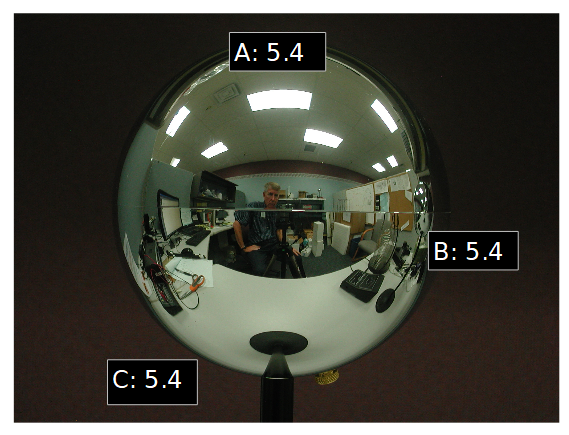
\includegraphics[width=0.6\textwidth]{anexos/esferaResultados.png}
    \caption{Distribución de carga en una esfera conductora. Los tres puntos A, B y C presentan lecturas similares (5.4 V), lo que indica una distribución uniforme de la carga en toda la superficie.}
    \label{fig:esfera}
\end{figure}

\begin{figure}[H]
    \centering
    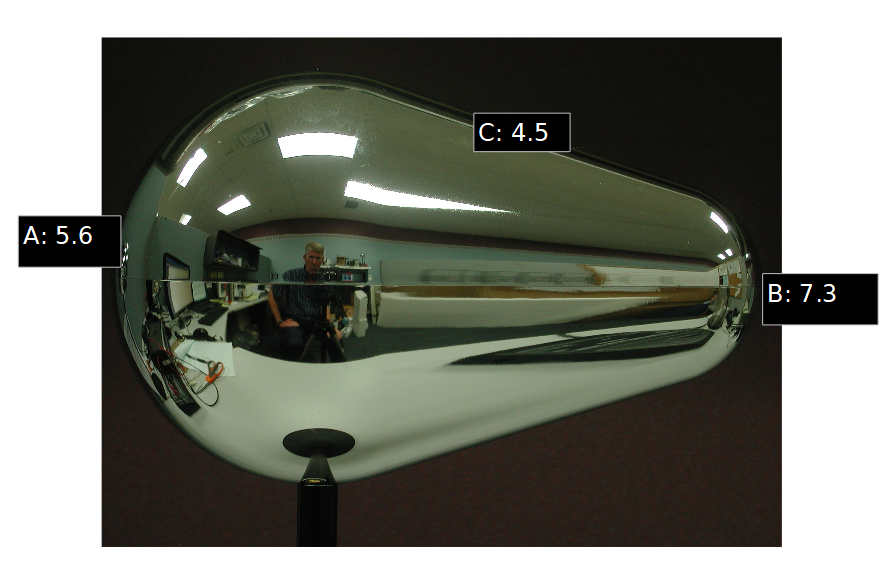
\includegraphics[width=0.8\textwidth]{anexos/gotaResultados.png}
    \caption{Distribución de carga en un conductor no esférico. Se observa que las regiones de mayor curvatura (punto B) concentran más carga (7.3 V), mientras que las zonas de menor curvatura (punto C) presentan menor potencial (4.5 V).}
    \label{fig:gota}
\end{figure}

En conjunto, los resultados experimentales concuerdan con las predicciones teóricas de la electrostática: la carga eléctrica se conserva durante los procesos de transferencia, se distribuye uniformemente en superficies equipotenciales y se concentra en los extremos o puntas de los conductores.

\paragraph{Observaciones --- Procedimiento B: Carga por contacto}

Luego de colocar el productor de carga blanca dentro de la canasta interior del cubo de Faraday,
la carga detectada fue de aproximadamente 60 V.
Esto indica que el disco blanco presentaba una carga inicial positiva, inducida por el frotamiento previo.

Después de permitir que el productor de carga blanca hiciera contacto con la pared interna de la canasta,
la lectura del electrómetro aumentó a 69 V, lo que confirma la transferencia parcial de carga al interior del conductor.

Finalmente, tras insertar el productor de carga oscura en la canasta interior y dejarlo en contacto con la pared,
la carga medida fue de -98 V, evidenciando que el disco oscuro poseía carga negativa y que, al tocar el conductor, transfirió electrones hacia la cesta, invirtiendo la polaridad respecto al caso anterior.

\paragraph{Observaciones --- Procedimiento C: Carga por inducción} 

Sin dejar que la varita toque el cubo de hielo: La polaridad de la carga en la varita blanca es positiva (+).

Después de conectar a tierra el cubo de hielo y retirar la varilla: La polaridad de la carga en el cubo es negativa (-), ya que al conectar a tierra, los electrones del sistema fluyen hacia el cubo atraídos por la varita positiva.

Repetición con el productor de carga oscura: La polaridad de la carga en la varita oscura es negativa (-).

Después de eso, la polaridad de la carga en el cubo es positiva (+), porque durante la conexión a tierra, los electrones fueron repelidos hacia la tierra debido a la presencia del campo negativo de la varita, dejando el cubo con carga neta positiva.

\paragraph{Preguntas --- Procedimiento C: Carga por inducción}
\begin{enumerate}
    \item \textbf{Al final del proceso, ¿cómo se compara la carga adquirida por el cubo con la polaridad de la carga en la varilla que se utilizó?}

    La carga adquirida por el cubo es de polaridad opuesta a la de la varilla utilizada.
    Durante la inducción, el campo eléctrico de la varilla provoca una separación de cargas en el cubo: las cargas de signo opuesto se atraen hacia el lado cercano a la varilla, mientras que las del mismo signo son repelidas. Al conectar a tierra el cubo, estas cargas del mismo signo se neutralizan o escapan, de modo que al retirar la conexión y la varilla, el cubo queda con una carga igual en magnitud pero opuesta en signo a la de la varilla inductora.

    \item \textbf{Al usar la varilla blanca: ¿El cubo de hielo ganó o perdió electrones durante la carga por inducción? ¿Adónde fueron (o de dónde vinieron) los electrones?}

    La varilla blanca tiene carga positiva, por lo tanto el cubo de hielo ganó electrones durante el proceso de inducción.
    Cuando el cubo se conectó a tierra, los electrones fluyeron desde la tierra hacia el cubo, atraídos por la carga positiva de la varilla. Una vez desconectado de tierra y retirada la varilla, esos electrones permanecieron en el cubo, dejando al conductor con una carga neta negativa.

    \item \textbf{Al usar la varita oscura: ¿El cubo de hielo ganó o perdió electrones durante la carga por inducción? ¿Adónde fueron (o de dónde vinieron) los electrones?}

    La varilla oscura tiene carga negativa, por lo que el cubo de hielo perdió electrones durante la inducción.
    En este caso, los electrones del cubo fueron repelidos hacia la tierra al establecer la conexión a tierra, debido a la repulsión del campo negativo de la varilla. Una vez retirada la conexión y el objeto cargado, el cubo quedó con deficiencia de electrones, es decir, con carga positiva.
\end{enumerate}


\section{Discusión y Conclusiones}
Los resultados experimentales obtenidos concuerdan con los principios teóricos de la electrostática. En la carga por frotamiento, se confirmó la transferencia de electrones entre las varillas, generando cargas de signo opuesto y demostrando la conservación de la carga total del sistema. En la carga por contacto, el cubo de Faraday adquirió la misma polaridad que el productor de carga, mientras que en la inducción obtuvo una carga opuesta, validando el efecto del campo eléctrico en la redistribución interna de cargas.

En el estudio de la distribución de la carga, las mediciones sobre la esfera conductora mostraron potenciales uniformes en todos los puntos, evidenciando que la carga se distribuye homogéneamente sobre la superficie externa. En contraste, el conductor no esférico presentó mayores potenciales en las zonas de mayor curvatura, verificando que la densidad superficial de carga aumenta en dichas regiones. Además, los ensayos con la esfera hueca confirmaron que el interior del conductor permanece eléctricamente neutro, en cumplimiento del principio de apantallamiento.

Posibles fuentes de error incluyen la presencia de humedad ambiental, cargas residuales en las varillas, y pérdidas por descarga en el aire. Aun así, las tendencias observadas son consistentes con la teoría.

En conclusión, se comprobó experimentalmente la ley de conservación de la carga, los mecanismos de electrización por frotamiento, contacto e inducción, y la distribución superficial de la carga en conductores, reafirmando los fundamentos de la electrostática.


% ----------------- Bibliografía -----------------
\begin{thebibliography}{9}

\bibitem{serway}
Raymond A. Serway, John W. Jewett Jr. (2017). \textit{Física para ciencias e ingeniería, Vol. II}. México: Cengage Learning.

\bibitem{pasco}
PASCO Scientific (2018). \textit{Práctico N°1: Cargas Electroestáticas}. Manual del Sistema de Laboratorio PASCO Capstone. Recuperado de la guía de laboratorio UTEC.

\bibitem{hyperphysics}
Nave, C. R. (2019). \textit{Electrostatics and Charge Distribution}. HyperPhysics, Georgia State University. Disponible en: \url{http://hyperphysics.phy-astr.gsu.edu/}


\end{thebibliography}

\end{document}
